\documentclass[11pt]{article}
\renewcommand{\baselinestretch}{1.05}
\usepackage{amsmath,amsthm,verbatim,amssymb,amsfonts,amscd, graphicx}
\usepackage{graphics}
\usepackage{tikz}
\usepackage[siunitx]{circuitikz}
\usepackage[utf8]{inputenc}
\usepackage[danish]{babel}
\topmargin0.0cm
\headheight0.0cm
\headsep0.0cm
\oddsidemargin0.0cm
\textheight23.0cm
\textwidth16.5cm
\footskip1.0cm
\usepackage{color}
\usepackage{listings}
\lstset{ %
language=VHDL,                % choose the language of the code
basicstyle=\footnotesize,       % the size of the fonts that are used for the code
numbers=left,                   % where to put the line-numbers
numberstyle=\footnotesize,      % the size of the fonts that are used for the line-numbers
stepnumber=1,                   % the step between two line-numbers. If it is 1 each line will be numbered
numbersep=5pt,                  % how far the line-numbers are from the code
backgroundcolor=\color{white},  % choose the background color. You must add \usepackage{color}
showspaces=false,               % show spaces adding particular underscores
showstringspaces=false,         % underline spaces within strings
showtabs=false,                 % show tabs within strings adding particular underscores
frame=single,           % adds a frame around the code
tabsize=2,          % sets default tabsize to 2 spaces
captionpos=b,           % sets the caption-position to bottom
breaklines=true,        % sets automatic line breaking
breakatwhitespace=false,    % sets if automatic breaks should only happen at whitespace
escapeinside={\%*}{*)},          % if you want to add a comment within your code
keywordstyle=\bfseries\color{blue!},
commentstyle=\itshape\color{green!},
identifierstyle=\color{red!},
stringstyle=\color{purple!},
}

\begin{document}
 
\title{Eksempler}

\author{Kristian Søgaard Søresen}

\maketitle



\section*{List}


\begin{lstlisting}
library ieee;
use ieee.std_logic_1164.all;

entity half_adder is						-- Initialising entity
	port (a, b : in std_logic;				-- Defining inputs
		sum, carry_out : out std_logic);	-- Defining outputs
end half_adder;

architecture dataflow2 of half_adder is		-- Architecture of half_adder
	begin
	sum <= a xor b;							-- (a xor b) is written to sum
	carry_out <= a and b;					-- (a and b) is written to carry_out
end dataflow2;
\end{lstlisting}

\section*{Tabel}

\begin{figure}[!ht]
    \centering
     \begin{tabular}{ l | l | l }
       Condition  & Invalid ECs       		    & Valid ECs     					 \\ \hline
       Row 	      &  $< 0[1]; < 15[2]$          & $0-15[3]$       				 \\
       Column     &  $< 0[4]; < 15[5]$          & $0-15[6]$  					 \\
       Tiles      &  $\in \{ mountains \} [7] $ & $ \notin \{ mountains \} [8]$  \\
       Unit       &  $> 1[9]; friendly unit[10]$& $ 1[11];0[12] $			     \\
       Unit action&  $moveUnit(fortify)$		& 
     \end{tabular}
    \caption{EC table of moveUnit}
\end{figure}

\section*{18W MOSFET}

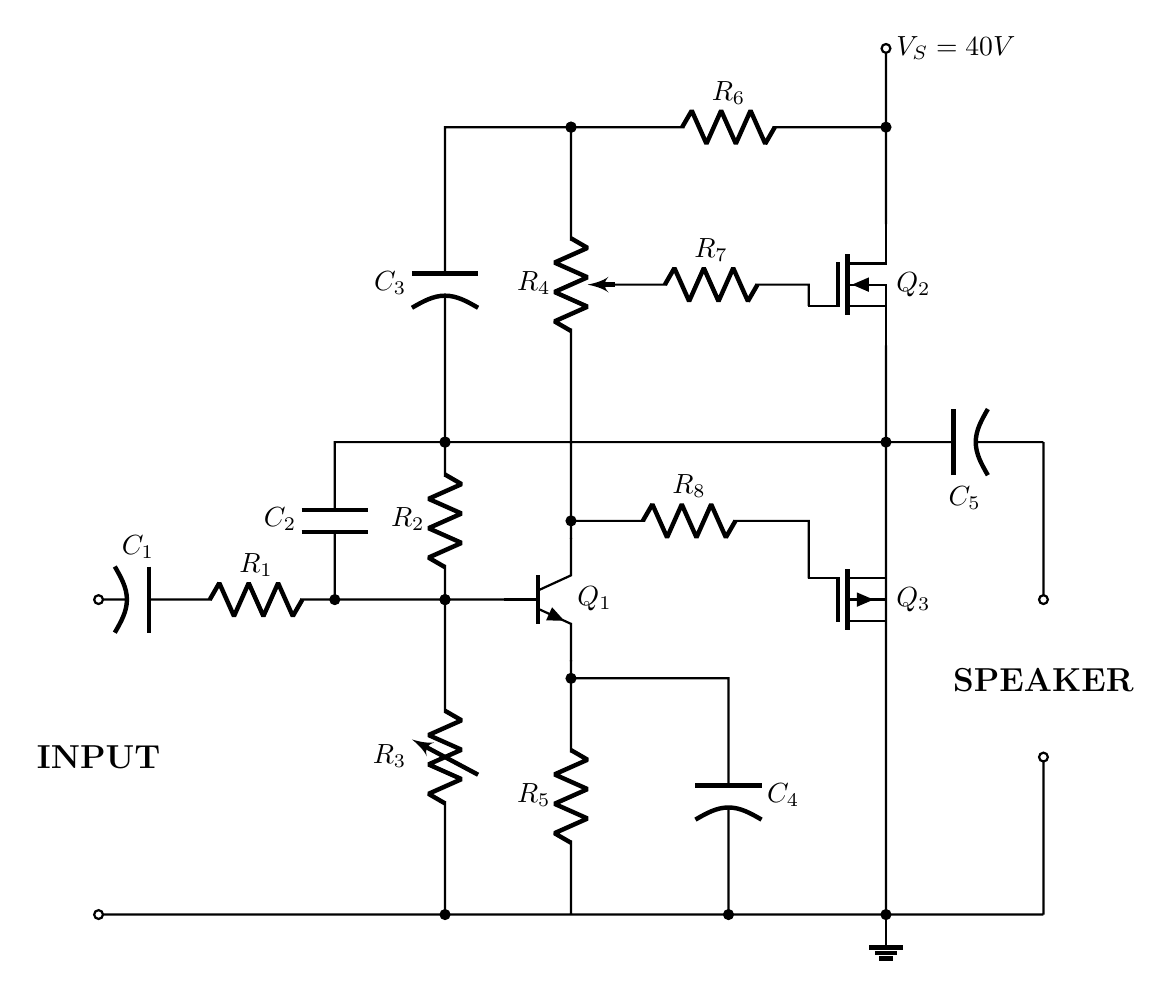
\begin{tikzpicture}[scale=2]
  \draw[color=black, thick]
    (0,0) to [short,o-] (6,0){} % Baseline for connection to ground
    % Input and ground
    (0,1) node[]{\large{\textbf{INPUT}}}
    % Connection of passive components
    (5,0) node[ground]{} node[circ](4.5,0){}
    (0,2) to [pC, l=$C_1$, o-] (0.5,2)
    to [R,l=$R_1$,](1.5,2)
    to node[short]{}(2.6,2)
    (1.5,2) to [C, l=$C_2$, *-] (1.5,3) -| (5,3)
    (2.2,2) to [R, l=$R_2$, *-*] (2.2,3)
    (2.2,3) to [pC, l=$C_3$, *-] (2.2,5) -| (3,5)
    % Transistor Bipolar Q1
    (3,0) to [R,l=$R_5$,-*] (3,1.5)
    to [Tnpn,n=npn1] (3,2.5)
    (npn1.E) node[right=3mm, above=5mm]{$Q_1$} % Labelling the NPN transistor
    (4,0) to [pC, l_=$C_4$, *-] (4, 1.5)--(3,1.5)
    (2.2,0) to [vR, l=$R_3$, *-*] (2.2,2)
    (3,2.5) to node[short]{}(3,3)
    (3,5) to [pR, n=pot1, l_=$R_4$, *-] (3,3)
    (3,5) to [R, l=$R_6$, *-] (5,5)
    to [short,*-o](5,5.5) node[right]{$V_S=40 V$}
    % Mosfet Transistors
    (5,3) to [Tnigfetd,n=mos1] (5,5)
    (mos1.B) node[anchor=west]{$Q_2$} % Labelling MOSFET Q2 Transistor
    (pot1.wiper)  to [R, l=$R_7$] (4.5,4) -| (mos1.G)
    (5,1.5) to [Tpigfetd,n=mos2] (5,2.5)
    (5,0) to (mos2.S)
    (3,2.5) to [R, l=$R_8$, *-] (4.5,2.5)
    -| (mos2.G)
    (mos2.B) node[anchor=west]{$Q_3$} % Labelling MOSFET Q3 Transistor
    % Output
    (6,3) to [pC, l=$C_5$,-*](5,3)
    (6,3) to [short,-o] (6,2){}
    (mos1.S)--(mos2.D)
    (6,0) to [short,-o] (6,1){} node[above=7mm]{\large{\textbf{SPEAKER}}}
    ;
\end{tikzpicture}

\section*{Graf}

\end{document}